\documentclass[12pt,a4paper]{report}
\usepackage[total={16.5cm,25.2cm}, top=2.5cm, left=2.5cm]{geometry}
\usepackage[czech]{babel}
\usepackage[T1]{fontenc}
\usepackage[utf8]{inputenc}
\usepackage{hyperref}
\usepackage{verbatim}
\usepackage{listings}
\usepackage{graphicx}
\usepackage{caption}
\graphicspath{ {./} }
\newcommand{\source}[1]{\caption*{Zdroj: {#1}} }
\setlength\parindent{0.5cm} % šířka odsazení prvního řádku odstavce
\linespread{1.25} % řádkování 1.5 dle MS Word


%%% Údaje o práci
% Název práce v jazyce práce (přesně podle zadání)
\def\NazevPrace{Funkcionální programování}
% Jméno autora
\def\AutorPrace{Ivan Žižka}
% Třída autora
\def\TridaAutora{8.M}
% Školní rok
\def\SkolniRok{2018/2019}
% Seminář ve kterém práce vznikla
\def\Seminar{Seminář z programování}
% Datum dokončení práce
\def\DatumDokonceni{22.2.2019}
\renewcommand\lstlistingname{}

%% Definice různých užitečných maker (viz popis uvnitř souboru)
%%% Tento soubor obsahuje definice různých užitečných maker a prostředí %%%
%%% Další makra připisujte sem, ať nepřekáží v ostatních souborech.     %%%

%%% Užitečné balíčky (jsou součástí běžných distribucí LaTeXu)
\usepackage{graphicx}       % vkládání obrázků
\usepackage{indentfirst}    % zavede odsazení 1. odstavce kapitoly
\usepackage[nottoc]{tocbibind} % zajistí přidání seznamu literatury,obrázků a tabulek do obsahu
\let\openright=\clearpage
\usepackage{hyperref}
\hypersetup{unicode}
\hypersetup{breaklinks=true}

%%% Drobné úpravy stylu

% Tato makra přesvědčují mírně ošklivým trikem LaTeX, aby hlavičky kapitol
% sázel příčetněji a nevynechával nad nimi spoustu místa. Směle ignorujte.
\makeatletter
\def\@makechapterhead#1{
  {\parindent \z@ \raggedright \normalfont
   \Huge\bfseries \thechapter. #1
   \par\nobreak
   \vskip 20\p@
}}
\def\@makeschapterhead#1{
  {\parindent \z@ \raggedright \normalfont
   \Huge\bfseries #1
   \par\nobreak
   \vskip 20\p@
}}
\makeatother

% Toto makro definuje kapitolu, která není očíslovaná, ale je uvedena v obsahu.
\def\chapwithtoc#1{
\chapter*{#1}
\addcontentsline{toc}{chapter}{#1}
}

% Trochu volnější nastavení dělení slov, než je default.
\lefthyphenmin=2
\righthyphenmin=2

% Zapne černé "slimáky" na koncích řádků, které přetekly, abychom si
% jich lépe všimli.
\overfullrule=1mm



\begin{document}

%% Titulní strana a různé povinné informační strany
%%% Titulní strana práce a další povinné informační strany

%%% Titulní strana práce

\pagestyle{empty}
\hypersetup{pageanchor=false}

\begin{center}

{\large\textbf{Gymnázium Christiana Dopplera, Zborovská 45, Praha 5}}

\vspace{70mm}

{\Large ROČNÍKOVÁ PRÁCE}
\\ \vspace{4mm}
{\Huge\bfseries\NazevPrace}

\vfill
\end{center}

\begin{tabular}{ll}
Vypracoval: & \AutorPrace \\
Třída: & \TridaAutora \\
Školní rok: & \SkolniRok \\
Seminář: & \Seminar \\
\end{tabular}
\newpage

%%% Strana s čestným prohlášením k diplomové práci
\openright
\hypersetup{pageanchor=true}
\pagestyle{plain}
\pagenumbering{gobble}
\vglue 0pt plus 1fill

\noindent
Prohlašuji, že jsem svou ročníkovou práci napsal samostatně a výhradně s~použitím citovaných pramenů. Souhlasím s~využíváním práce na Gymnáziu Christiana Dopplera pro studijní účely.
\vspace{10mm}

\noindent V Praze dne \DatumDokonceni
\hfill
\AutorPrace

\vspace{20mm}
\newpage
\noindent
{\LARGE\textbf{Poděkování}}

\vspace{10mm}
Chtěla bych poděkovat Mgr. Janu Hamáčkovi za vedení mé práce, rady a věcné připomínky. Dále bych chtěl poděkovat RnDr. Rudolfovi Krylovi za odbornou konzultaci při zpracování této práce. 
\newpage

\openright
\pagestyle{plain}
\pagenumbering{arabic}
\setcounter{page}{3}


%%% Strana s automaticky generovaným obsahem diplomové práce

\tableofcontents

\chapter{Úvod}
Cílem práce je vytvořit dva programy s identickou funkcí, ale každý vytvořený v jiném programovacím jazyce a zcela jinou metodou. Oba programy budou převádět prefixový zápis na infixový s tím ,že první z~těchto dvou bude tvořen procedurálně a~to v~jazyce C. Druhý program bude tvořen v čistě funkcionálním programovacím jazyce Haskell. Hlavním cílem je srovnat odlišné styly programování a zároveň ukázat výhody a nevýhody funkcionálních programovacích jazyků. 

\chapter{Teorie funkcionálního programování} % NÁZVY KAPITOL NEJVYŠŠÍ ÚROVNĚ

\section{Historie}
Čistě funkcionální programovací jazyky vycházejí z konceptu, který navrhl ve 30. letech 20. století britský matematik Alonzo Church. Ten vytvořil lambda kalkul jakožto matematickou teorii funkcí. Church vytvořil také jednu z nejvýznamnějších tezí celého funkcionálního programování, tato teze se nazývá Church-Turingova teze. \cite{Funk. prog. wiki.} Tato teze srovnává člověka, který následuje algoritmus, a Turingův stroj.

Lambda kalkul je čistě teoretický model, ale i tak na něm staví většina čistě funkcionálních programovacích jazyků. Lambda kalkul analyzuje funkci a nikoliv z hlediska původního matematického smyslu zobrazení z množiny, ale jako metodu výpočtu. \cite{lambda kalkul wiki.} Lambda kalkul tvoří páteř takzvaných Turingových strojů. Občas je označována jako univerzální matematický programovací jazyk.

Prvním jazykem, který obsahoval funkcionální část byl LISP, který byl vytvořen pro potřeby IBM v 50. letech minulého století. LISP se dodnes vyučuje na většině vysokých škol v~USA, které se zaměřují na studium informatiky, a je brán za jednu z nejdůležitějších schopností každého absolventa takovéto vysoké školy. Prvním čistě funkcionálním programovacím jazykem byla Miranda, tento jazyk byl vyvinut Davidem Turnerem. Byl komerčně podporován a snažil se odpoutat od závislosti na jiných programovacích jazycích. Krátce po vydání jazyku Miranda, proběhla světová konference o funkcionálním programování, ze které vzešel požadavek na standardizaci funkcionálních programovacích jazyků. \cite{Funk. prog. wiki.} Z tohoto důvodu byla sestavena speciální komise, která vyprodukovala čistě funkcionální programovací jazyk Haskell. 

\section{Funkcionální programování}
Funkcionální programování se spíše než klasickým programovacím jazykům podobá matematickému zápisu funkce. Hlavní princip je založen na zápisu programu ve tvaru výrazu. Ten je následně zjednodušován až do takové míry, kdy už nelze být zjednodušen. Tento tvar je výsledkem tohoto výrazu. \newline
Příklad: \newline
$(2 * 5)$ Tento výraz není nic jiného než funkce násobení (ta vyžaduje dva argumenty, které mezi sebou vynásobí), jehož výsledkem je číslo 10. Číslo 10 nelze dále zjednodušit a proto považujeme tento výraz za výsledek. 

Program lze, a dokonce je to vyžadováno, dělit do funkcí. V deklarativním programování mohou funkce přijímat jako argument jiné funkce. To zajišťuje plynulost a absenci pomocných proměnných. Funkce často obsahují jen několik řádků kódu. Zajímavou vlastností funkcionálních jazyků je pohled na funkce jako takové. Ty jsou chápány jako proměnné v imperativních programovacích jazycích. Například v jazyku C, pokud nebereme v potaz ukazatele, je zcela nemyslitelné vytvořit pole funkcí. Na druhou stranu ve funkcionálním programovaní je tato myšlenka naprosto validní a uskutečnitelná.  

\subsection{Rozdíl mezi funkcionálním a imperativním programováním}
Základní jednotkou funkcionálních jazyků je výraz. Ten se dále zjednodušuje až do té doby, kdy ho nelze dále zjednodušit. 

Na druhou stranu u imperativních jazyků je základní jednotkou příkaz. Rozdílem je, že tyto příkazy nemají obvykle argument (hodnotu). Proto způsobem, jakým si příkazy vyměňují data, musí být skrze proměnnou. Proměnnou se rozumí stavový vektor, který lze v~průběhu běhu programu měnit, hodnota vektoru je dána během programu. Existencí stavů vzniká jeden závažný důsledek.
\newline
\newline
Příklad:\newline
Funkce sum, která pro každé celé kladné číslo \textit{n} spočítá součet všech čísel od nuly do čísla \textit{n} .\newline
\begin{lstlisting}[caption={jazyk C}, captionpos=b, language = C]	
int sum (int n) {
  int i;
  int s = 0;
  for (i = n; i >= 0; i --)
    {
    s = s + i;
    }   
  return s;
}
\end{lstlisting}

Důsledkem tohoto programování je změna proměnných \textit{i} a \textit{s} v průběhu chodu programu. Při každém otočení cyklu se změní hodnota \textit{i} a \textit{s}.
 
U funkcionálních jazyků se tato vlastnost nevyskytuje. To je dáno z deklarace čistě funkcionálních jazyků, kde jestliže se ve stejném kontextu vyskytuje tentýž výraz, tak bude mít vždy stejný výsledek. %[http://programujte.com/clanek/2006032503-co-je-to-funkcionalni-programovani/]
Tuto vlastnost nazýváme referenční transparentnost.

\begin{lstlisting}[caption={jazyk Haskell}, captionpos=b, language=Haskell]	
sum :: Int -> Int
sum n = if n == 1 then 1 else n + sum (n - 1)
\end{lstlisting} 

\newpage
Na tomto příkladu můžeme vidět, že \textit{n} bude v určitém kontextu existovat jen jedno a~bude neměnné. I~kdybychom chtěli v~průběhu programu změnit hodnotu \textit{n}, tak nemůžeme. Deklarativní jazyky nemají prostředek, který by jim tuto manipulaci zajistil. Mohli bychom namítnout, že při vynořování z funkce $sum$ se mění hodnota proměnné \textit{n}. Opak je ale pravdou, ve funkci $sum$ existuje vždy jen jedno konkrétní \textit{n}, které má s předchozím n společný jen název, ale jeho hodnota je jiná.

Zajímavou vlastností imperativních jazyků je například to, že v nich můžeme simulovat podobné procesy jako v deklarativních jazycích. \newline
Příklad:

\begin{lstlisting}[caption={jazyk C}, captionpos=b, language = C]	
int sum(int n){
    int souc;
    if( n == 1 ){
        return 1;
    }
    else{
        souc = n + sum( n - 1 );
    }
return souc;
\end{lstlisting} 

I když je tato funkce napsána v imperativním jazyce, tak v ní probíhá stejná posloupnost akcí jako u příkladu s funkcionálním jazykem. Nefunkcionální jazyky mají prostředky, kterými lze simulovat chování funkcionálních jazyků, ale ne všechny funkce se takto dají simulovat. 

Deklarativní jazyky neznají pojem proměnné ani přiřazení do ní. Proměnné mohou být pouze vázány na argumenty funkcí. To znamená, že argumentem funkce $sum$ může být výraz: $(5 + 7)$ ten je následně vázán na argument funkce \textit{n}. Z tohoto důvodu můžeme říci, že $n = 5 + 7$, ale nejedná se v tomto případě o proměnnou. Vazbě na argument funkce se říká prostředí. V některých případech může absence stavových vektorů vest ke zkrácení řešení určitého problému.

\subsection{Lambda kalkul}
Základní prvky tohoto univerzálního matematického jazyka jsou tři: proměnná, aplikace a abstrakce. Proměnná je název pro hodnotu, kterou nelze blíže specifikovat. Jsou označeny identifikátory, často to jsou písmena abecedy. %[citace - http://www.cs.vsb.cz/navrat/vyuka/flp/texty/fp/ch02.html 
Abstrakce, je definice funkce. Zapsání takovéto abstrakce si lze nejlépe představit na příkladu: $f(x) = x - 5$, tuto funkci můžeme také zapsat pomocí lambda kalkulu $\lambda x.x - 5 $. \cite{volné a vázané} Výraz (proměnná) mezi $\lambda$ a \textit{.} je parametr funkce, parametrů může být i více, ale v tomto případě máme jen jeden. Výraz za tečkou značí definici funkce (tělo). 

Problém nastává, když máme právě více parametrů než jeden. Jelikož lambda kalkul dokáže operovat pouze s~jednou. I tento problém je jednoduše řešitelný, například funkci o~dvou parametrech, která má předpis: $g(x,y) = x * y$  můžeme zcela beztrestně přepsat takto: $\lambda x. \lambda y. x * y $ tento zápis je možno zkrátit na: $\lambda x \; y.\ x * y $. Aplikace, toto je výraz pro volání funkce - $f(x) = x - 5$. Například funkci \textit{f} zavoláme s parametrem $5$, čili se za proměnnou \textit{x} dosadí číslo $5$. Výsledkem této funkce bude $0$. Když se koukneme na volání funkce z blízka, tak zjistíme ,že nejdříve je volána funkce \textit{f} a následně argument $5$. Tento postup se též dá zapsat jako $(\lambda x.x - 5) \;5$  

Často se tyto tři pojmy schovají za značení \textit{E}. 
\subsubsection{Vázané a volné proměnné}
Proměnná je v $\lambda$-výrazu vázaná, pokud se jedná o parametr nějaké funkce, takže např. ve výrazu $ (\; \lambda x . \; y\; x\; )$ je \textit{x} vázaná proměnná. \cite{volné a vázané} Protikladem k~vázané proměnné je volná, například: $(\; \lambda x . \; y\; x\; )$. Zde je \textit{y} volnou proměnnou. Obecně řečeno proměnná se vždy váže k~nejbližší lambdě ~k~ní vlevo. V~lambda výrazech je nutno respektovat závorky, ty určují nejen oddělení parametru, ale také říkají, ke které lambdě se proměnná bude vázat. To si lze jednoduše představit na příkladu: $ ( \; \lambda x . \; (\lambda x .\; x - 2)\; z\; ) $~, kde \textit{x} je proměnná vázaná a~\textit{z}~proměnnou volnou. Taktéž \textit{x} se váže~k~$\lambda$, které je v~závorce s~ním. 

\subsection{Higher-order funkce}
Tímto pojmem se označují takové funkce, které splňují alespoň jednu ze dvou podmínek:
\begin{enumerate}
\item funkce může přijímat jako argument jinou funkci
\item výsledkem této funkce může být jiná funkce
\end{enumerate}
Příklad, který je nám blízký, můžeme nalézt v matematice a to u funkcí derivace a integrace. Tyto funkce mají za argument jinou funkci a výsledkem je funkce, která vychází z původního argumentu.   

Příkladem takovéto funkce může být (v Haskellu) funkce $ map $, která vyžaduje dva argumenty, z níž je jeden funkce \textit{f} a druhý list \textit{l}. Výsledkem je list, na který byla aplikována funkce \textit{f}.
\newpage
\subsection{Vedlejší efekty}
Nastávají tehdy, kdy funkce během výpočtu mění stav procesu, než je návratová hodnota funkce. Vedlejší efekty jsou častým zdrojem chyb v kódu, na druhou stranu může správně použitý vedlejší efekt usnadnit implementaci kódu. 

Příkladem neúmyslného vedlejšího efektu může být toto:
\begin{lstlisting}[caption={jazyk C}, captionpos=b, language = C]	
void and(int a, int b)
	{
	int sum = a + b;	
	printf("%d", sum);	
	return;
}

int main(){
	int n = 1;
	add(n++, n);	
	return 0;
}
\end{lstlisting} 
Zde se jedná o zcela zjevný vnější efekt. Jelikož nevíme jestli se zavolá funkce \textit{add} s argumenty \textit{2 a 1} nebo s argumenty \textit{2 a 2}. Toto rozhodnutí leží na konkrétním překladači a dokumentaci daného jazyka. V tomto případě se vypíše číslo: $3$. 

Úmyslným použitím vedlejšího efektu může být funkce \textit{sleep(500)}, která nám na základě hardwarového času uspí program.

Obecně se může říci, že za vedlejší efekty můžeme považovat změnu hodnoty proměnné, ukládání na disk nebo načítání vstupu.   
\subsection{Monády}
Monády jsou druhem abstrakce datového konstruktoru (type class), tyto konstruktory uzavírají určitou část logiky programu. Monády umožňují programátorovi vytvářet složité funkce, tím je myšleno řetězení funkcí. V minimalistickém principu jde o programovou strukturu, která umožňuje určitý výpočet. Monády jsou často zaváděny z důvodu toho, aby se předešlo vedlejším efektům funkcí. 

Čistě obecně jde o konstrukci na úrovni teorie kategorií. Důležité je zmínit, že monády jsou často použity v kódu, aniž bychom si to uvědomovali. Jedno z takových užití je řešení vstupu a výstupu programu, například do konzole. Myšlenka za touto funkcí je taková, že funkci IO je předáván stav programu jako argument (stav = momentální vyhodnocení výrazu programem). IO následně například vypíše daný výsledek do konzole. Mohlo by se zdát, že se jedná o jakési implementování vlastností z imperativních programovacích jazyků. Není tomu tak vždy, jen v kontextu IO se tato představa nabízí. Monády jsou zárukou toho, že je zachována čistá funkcionalita jazyka bez vedlejších efektů, ale zároveň nám umožňují využívat vlastností, které mají vedlejší efekty. 

Třída monád, podporuje dva operátory jeden z nich je operátor \texttt{bind}, ten se značí $ (>>=) $ a druhou \texttt{return} ten vrací monádu. 
\subsubsection{IO - vstup a výstup}
Touto funkcí se rozumí monadická funkce, která může být použita různými způsoby. Prvním z nich je IO s datovým typem například: \textit{IO Char}. Druhým způsobem použití může být \textit{IO()} takto definovaná funkce nevrací žádnou hodnotu. Práce ve funkci, která je definována pomocí \textit{IO()}, musí probíhat až za klíčovým slovem \textit{do}. Toho se dá využít například při načítání ze souboru nebo vypisování do konzole.  

\subsubsection{Maybe}
Monáda \textit{Maybe} má tu vlastnost, že dokáže vracet dva různé výstupy, jedním z nich je \textit{Just x} a druhým \textit{Nothing}. Je definována takto:

\begin{lstlisting}[language=Haskell, caption={Definice Maybe}, captionpos=b,]
data Maybe x = Just x | Nothing
return x = Just x
Nothing >>= f = Nothing	
Just x >>= f = f x
\end{lstlisting}
Je-li výstupem funkce \textit{f - Nothing}, tak se vypíše jen \textit{Nothing}, jeli výsledkem funkce validní výsledek přidá se před tento výsledek \textit{Just}. Funkce \textit{return} vrací ono \textit{Just x} zpět.\cite{monady} Důležité k~této definici je zmínit to, že \textit{x} může být jakéhokoliv typu.  

\subsubsection{List}
I list, který je jedním z nejpoužívanějších vlastností Haskllu, je monáda. List je definován takto:
\begin{lstlisting}[language=Haskell, caption={Definice List}, captionpos=b,]
return x = [x]
xs >>= f = concatMap f xs 
\end{lstlisting}
Když by byl zadán jen jeden prvek, funkce \textit{return} vrátí jednoprvkový list. Další řádek definice je o trošku zajímavější, tento kus definice se stará o to, aby všechny prvky byly vypsány v~listu. Toho je docíleno tak, že na každý prvek je volána funkce \textit{f} a~následně funkcí \textit{concat} jsou všechny prvky sloučeny do jednoho listu.  

\section{Haskell}
Tento programovací jazyk řadíme do kategorie jazyků s líným vyhodnocováním.\cite{haskell} Což znamená, že program vyhodnotí funkci nebo výraz jen v tom případě, že je nutná k dosažení konečného výsledku. Haskell také pečlivě lpí na mezerách, které mají syntaktický význam. Existují dva hlavní kompilátory pro Haskell, prvním z nich je Hugs -- v dnešní době se již moc nepoužívá. Druhým, ale daleko významnějším kompilátorem je GHC = Glasgow Haskell Compiler. Tento kompilátor je multiplatformní a velmi dobře aktualizován. Operátory funkcí se chovají stejně jako v matematice, existuje zde několik možných zápisů. Prvním z nich je infixový tvar [ 8 `mod` 2 -- ukázka infixu ], který je nutné ohraničit zpětným apostrofem. Dalším způsobem je prefixový tvar [ mod 8 2 -- ukázka prefixu ], zde si lze lépe představit, že funkci \textbf{mod} jsou předány dva argumenty ( 8 a 2 ). Volba zápisu je samozřejmě možná i~u~základních operací jako jsou například sčítaní nebo odčítání. Haskell dokáže velice dobře vyhodnocovat prioritu operací, také platí, že volání funkce má přednost před operací. Prioritu operací můžeme upravovat pomocí závorek. Syntax tohoto programovacího jazyka je velice striktní v~pojmenovávání funkcí, proměnných a~datových typů:
\begin{itemize}
\item funkce se značí malými písmeny 
\item datové typy se značí prvním velkým písmenem (např: String, Char)
\item proměnné (nemění se = vstup) se značí stejně jako funkce malým písmenem
\end{itemize}

\newpage 
\chapter{Aritmetické výrazy}            
\section{Notace}
\subsection{Prefix}
Prefixová notace, v některé literatuře zvaná též polská notace, je varianta zápisu algebraických výrazů. V této variantě se operátory zapisují před operandy. Protože je pořadí operátorů fixní, syntaxe nepotřebuje žádné závorky a zápis je tedy jednoznačný. \cite{prefix}
Tento způsob je velice oblíbený v informatice, jelikož jeho vyhodnocení trvá lineární množství času a je poměrně jednoduché. 


K vyhodnocení využíváme zásobník (stack) - do tohoto zásobníku postupně vkládáme celý výraz zprava doleva: $+\;26\; * \;3\;\; 6\;$

Do zásobníku se nejdříve vloží číslo 6, následně se vloží číslo 3, jako další by se měl vložit operátor *, ale místo toho se tato operace (~*~) provede na poslední dva členy v zásobníku (jsou vyjmuty ze zásobníku) a výsledek operace $3*6 = 18$ je uložen opět do stejného zásobníku. V dalším kroku je do zásobníku vloženo číslo 26 a poté operátor +. Operace (~+~) se provede opět na poslední dva členy v zásobníku (26~+~18) a výsledek je opět uložen do zásobníku. Výraz je vyhodnocen tehdy, když v zásobníku zůstane jen jediná hodnota, která je výsledkem výrazu. 
\subsection{Postfix}
Postfix je velice podobný prefixu. Jak již název napovídá jedná se o zápis, kde se operátory píší za operandy. Stejně jako u polské notace není důležité používat závorky, jelikož pozice operátorů je fixní. 
Vyhodnocení probíhá naprosto stejně jako u polské notace, ale s tím rozdílem, že čteme výraz zleva doprava. Vkládáme je do zásobníku a provádíme na nich operace, mezivýsledky následně taktéž vkládáme do zásobníku. \newline
Příklad postfixového zápisu: $ 5 \;\;1 \;\;2\;\; +\;\; 4\;\; *\;\; +\;\; 3\;\; -\;\; $
\newline
Výhodou může být jednoduchost vyhodnocení, čtení zleva doprava, rychlost vyhodnocení.\newline
Nevýhodami jsou neintuitivnost zápisu výrazu a dodržování mezer.
\subsection{Infix}
Infixová notace je běžný způsob zápisu výrazu ve vzdělávacích systémech a i v běžném 
životě. Je velice intuitivní a jednoduše čitelný. Operátory se píší mezi operandy, z toho 
vyplývá nutnost používání závorek, když chybí závorky je priorita operací zřízena operátory. I když je pro člověka tato notace velice jednoduchá, tak pro počítačové zpracování není. Je tu hned několik možností vyhodnocení tohoto výrazu. Jedním z možností je převést infixový tvar na postfixový nebo prefixový. Toho lze dosáhnout za pomoci Shunting-yard \cite{výrazy} algoritmu a následně velice jednoduše vyhodnotit tento nový zápis. Další možností je vyhodnocení pomocí formálních gramatik, tento způsob je například využíván operačními systémy. Třetí způsob je převedení výrazu do binárního stromu, kde každý otec je znaménko a jeho poslední syn je vždy číslo. Následně je výraz vyhodnocen rekurzivně. 
\newline
\newline
Teorie převedení výrazu zapsaného v infixové podobě: 
\newline
Strom je tvořen pouze operátory a operandy. V první fázi, musí program najít operaci s~nejnižší prioritou, při tomto procesu musí respektovat pořadí operandů, ale také rozmístění závorek. Když takovou operaci nalezne, stává se toto znaménko s nejnižší prioritou dělící čarou, která rozděluje výraz na dvě podmnožiny. Stejná funkce je zavolána na obě vzniklé části a~celý proces pokračuje, dokud nezůstane jen jedna operace mezi dvěma operandy. Strom je stavěn rekurzivně s~tím, že se do každého otce (pokud má syny) je uloženo znaménko (operátor). Do otců, které nemají žádné syny jsou uloženy operandy. Ukázka stromu pro výraz $\;\;3\;+\;(\;(\;5\;+\;9\;)\;*\;2\;)\;\;$ je vidět v následujícím obrázku (Binární strom).

\begin{figure}[h]
    \centering
    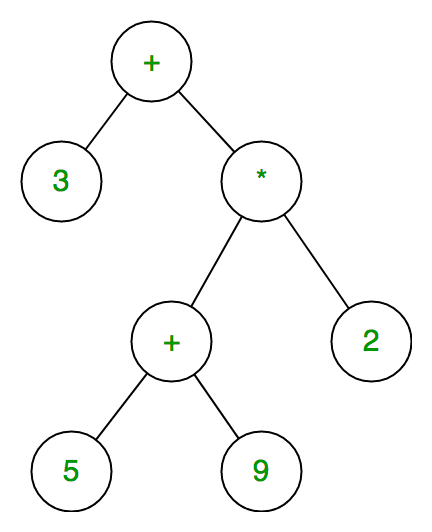
\includegraphics[scale = 0.4]{expression-tree}
    \caption{Binární strom}
	\source{\url {https://www.geeksforgeeks.org/expression-tree}}   

\end{figure}
\newpage 
\subsubsection{Převod notací} 
Převod notací z binárního stromu je velice jednoduchá záležitost, závisí na pořadí výpisu synů a otce. \newline
\textbf{Převod z infixu na postfix:} \newline
Za pomocí rekurze se vypíše nejdříve levý syn, následně pravý syn a nakonec otec těchto synů.\newline
\textbf{Převod z infixu na prefix:} \newline
Za pomocí rekurze se vypíše nejdříve otec, následně levý syn a nakonec pravý syn. Jelikož v~tomto typu zápisu nejsou vyžadovány závorky, je takto vzniklý výraz validní.\newline
\textbf{Převod z binárního stromu zpět na infixový zápis:}\newline
Opět za pomoci rekurze vypíšeme vždy nejdříve levého syna, následně otce a poté pravého syna. Před každým vypsáním levého syna vypíšeme závorku a po každém vypsání pravého syna ukončíme tuto závorku. Tím nám vznikne původní výraz, který bude obsahovat více závorek nežli původní, ale výsledek výrazu zůstane nezměněn. 

\chapter{Dokumentace}
Oba níže popsané programy mají stejnou funkci, převádějí prefixovou notaci na infixovou. Toho docilují za pomoci binárních nevybalancovaných stromů, které jsme si představili výše.

Ten jen postaven z prefixové notace. Stavba probíhá pomocí rekurze, která se zanořuje pokaždé, když je načteno znaménko. Znaménka jsou vždy otcové a čísla výhradně syny, kteří nemají potomky.

Důležitou věcí, která je potřeba zmínit, je ta že oba programy jsou přizpůsobeny na převádění výrazů, které obsahují pouze \textbf{jednociferná čísla}. 

\subsection*{Získání zdrojového kódu}
Existují dvě cesty jak lze získat zdrojový kód. První možností je přistoupit na url adresu (viz. příloha ), zde kliknout na tlačítko \textit{Clone or download}, a následně vybrat možnost \textit{Download ZIP}. Tento soubor je poté nutno extrahovat. 

Druhou možností je využití nástroje \textit{Git}. Zde je opět nutné přejít na url adresu (viz. příloha), zde kliknout na tlačítko \textit{Clone or download} a následně zkopírovat odkaz, který se nachází v nově vzniklém boxu. Poté je nutné se přesunout do vašeho počítače, ve kterém je nainstalován program \textit{Git}. Otevřít konzoli Git (\textit{Git Bash}), zde je nutné se navigovat do složky, kam chcete uložit repositář, a~poté užít příkaz \textit{git clone (adresa, kterou jsme si již dříve zkopírovali)}.

V tuto chvíli máte přístup ke zdrojovému kódu jednotlivých programů.   

\section{Dokumentace procedurálního programu}

\subsection{Vývoj a editace}
Program byl vyvíjen v nástroji \textit{Code Blocks}, v repositáři se nachází nastavený projekt. Editace vstupu probíhá přímo v~kódu, v~souboru \textit{main.c}. Rozhodli jsme se zvolit tento, ne až tak praktický způsob, jelikož jsme chtěli primárně ukázat rozdíl mezi imperativním a~neimperativním způsobem programování. 
\newpage
\subsection{Princip fungování}
Program vezme vstup, který mu zadal uživatel (modifikoval pole \textit{vstupniData}), převede ho do pole datového typu \textit{prefix}. Datový typ prefix obsahuje dvě proměnné z~nichž první je znak a~druhá číslo. Pokud je zadáno číslo, znak má nastavenou hodnotu na \textit{NULL}. Tento výše popsaný proces se děje pomocí funkce \textit{poleDoPrefix} (viz strana \pageref{pDP}.).

Ve funkci \textit{main} je následně vytvořena hlava stromu (datový typ \textit{strom}) a její všechny části jsou nastaveny na \textit{NULL}. Poté je volána funkce \textit{UkladaniDoStromu} (viz strana \pageref{UDS}.),~která zajišťuje inicializaci stavby stromu.

Po ukončení stavby stromu je zavolána funkce \textit{infix} (viz strana \pageref{infix}.), která vypíše do konzole infixový tvar. 


\subsubsection{poleDoPrefix} \label{pDP}
Tato funkce vyžaduje dva argumenty, prvním z nich je vstupní pole (zadaná data) a druhým argumentem je počet prvků pole, ten je získán podílem, kde prvním operandem je velikost vstupního pole a druhým je velikost datového typu \textit{char}. Výstupem funkce \textit{poleDoPrefix} je ukazatel na  pole datového typu \textit{prefix}.

\subsubsection{UkladaniDoStromu} \label{UDS}
Inicializuje ukládání do stromu, tím že kontroluje, jestli nebyl zadán prázdný vstup a následně volá funkci \textit{ZapisDoLeva} (viz strana \pageref{ZDL}.). Argumenty funkce \textit{UkladaniDoStromu} jsou vstupní data (datový typ prefix), ukazatel na hlavu (datový typ strom) a velikost pole (datový typ int). Výstupem není nic, jelikož ukazatel na hlavu stromu si uchováváme ve funkci \textit{main}.

\subsubsection{ZapisDoLeva} \label{ZDL}
Argumenty této funkce jsou: ukazatel na hlavu, vstupní pole a index (ten říká kolikáté pole vstupních dat se má uložit do stromu). Funkce si následně vytvoří proměnnou syn, která je ukazatelem na datový typ \textit{strom} (viz strana \pageref{strom}.). Poté je kontrolováno, zda se má uložit znaménko či číslo. Pokud se jedná o znaménko je do struktury \textit{syn} uloženo a pomocí ukazatelů je vytvořen odkaz z otce na syna a opačně. Následně je rekurzivně volána opět funkce \textit{ZapisDoLeva} s vyšším indexem o jedna. 

Jedná-li se o číslo, je uloženo do struktury a opět je vytvořeno propojení mezi otcem a synem. Poté je zavolána funkce \textit{ZapisDoPrava} (viz strana \pageref{ZDP}.), ale je jí předán odkaz na otce. 
\newpage
\subsubsection{ZapisDoPrava} \label{ZDP}
V principu funguje stejně jako předchozí funkce, akorát s tím rozdílem, že pokud se jedná o znaménko netypicky volá funkci \textit{ZapisDoLeva}.  

V případě, že se jedná o číslo provede naprosto stejné kroky, jako funkce  \textit{ZapisDoLeva}, ale rozdílem je to, že funkci \textit{ZapisDoPrava} je předán ukazatel na otce otce syna (Otec->Otec).


\subsubsection{strom} \label{strom}
Základní stavební jednotkou celého programu je struktura \textit{strom}. Ta tvoří základ aritmetického stromu, obsahuje ukazatel na levého a pravého syna, ukazatel na svého otce a~dvě proměnné, které uchovávají znaménko nebo číslo. Pokud ukazatel nikam nevede, je mu nastavena hodnota \textit{NULL}. Příkladem může být ukazatel na otce u kořene celého stromu. Ten logicky nikam nevede, a~tak je nastavena hodnota \textit{NULL}. 

\subsubsection{infix} \label{infix}
Funkce inicializuje vypsání infixového tvaru výrazu. To je zajištěno tím, že vypíše nejdříve levou větev (\textit{vypisL} viz strana \pageref{vL}.) a následně pravou (\textit{vypisR} viz strana \pageref{vR}.). Mezi ně je vypsáno znaménko.

\subsubsection{vypisL} \label{vL}
Pokud je v hlavě (ta je předána v argumentu) znaménko, zavolá se funkce \textit{vypisL}, poté se vypíše znaménko v hlavě a následně se volá funkce \textit{vypisR}. 

Je-li v hlavě uloženo číslo, vypíše se začátek závorky a následně toto číslo. 

\subsubsection{vypisR} \label{vR}
Pokud je v hlavě (ta je předána v argumentu) znaménko, zavolá se funkce \textit{vypisL}, poté se vypíše znaménko v hlavě a následně se volá funkce \textit{vypisR}. 

Je-li v hlavě uloženo číslo, vypíše se toto číslo a následně konec závorky.
\newpage
\section{Dokumentace neprocedurálního programu}
\subsection{Vývoj a editace}
Program byl vyvíjen v jazyce Haskell na platformě linux, jako vývojové prostředí jsme zvolili Atom. Hlavním důvodem bylo to, že existuje velké množství doplňků, které například zvýrazňují syntax Haskellu. Další nástroj, který je nutný pro kompilaci programu, je \textit{stack}. Který je dostupný z oficiálních stránek Haskellu \cite{stack}, ten obsahuje nástroj pro vytváření projektů, je schopen automaticky stahovat velké množství knihoven a navíc již sám o sobě obsahuje nejpoužívanější knihovny.
 
Editace je možná přímo v souboru \textit{Main.hs}, proč tomu tak je jsme již vysvětlili.  

\subsection{Spuštění a kompilace}
Pokud se rozhodneme spustit program na platformě Windows a máme již nainstalován kompilátor i s doplňky, stačí jen otevřít složku \textit{App}, v ní spustit soubor \textbf{Main.hs} a napsat příkaz \textbf{main}. Tím se spustí hlavní funkce programu a vypíše se výsledek. Pokud budeme editovat vstupní data, stačí upravenou verzi jen uložit a kompilátor sám zkompiluje daný program. 
 
\subsection{Princip fungování}
Ve funkci \textit{main} je volána funkce \textit{printIndex}, jejíž argumentem je další funkce. Tato funkce je \textit{buildTree} (viz strana \pageref{buildTree}.) s~argumentem \textit{prefix}.

Již z definice Haskellu víme, že program začne vyhodnocovat nejdříve funkci \textit{buildTree} a následně vyhodnotí funkci \textit{printIndex} s argumentem, který je roven výsledku \textit{buildTree}. Tímto argumentem bude datová struktura stromu. Následně může být vypsán infixový tvar výrazu.  

\subsubsection{buildTree} \label{buildTree}
Funkce nejdříve postaví levou (\textit{buildLeft} viz strana \pageref{buildLeft}.) část stromu a následně pravou část  (\textit{buildRight} viz strana \pageref{buildRight}.). Výstupem této funkce je datový typ Tree Char. Argumentem, který dostává je list znaků, v programu zvaný \textit{prefix}.

\subsubsection{buildLeft} \label{buildLeft}
Dostává dva argumenty, jedním z nich je list znaků (\textit{prefix}) a druhým je pomocný datový typ Builder Char (viz strana \pageref{Builder}.). Ten zajišťuje to, aby byl vždy vzat správný prvek z listu. Dalším důvodem jeho použití je to, že si dokáže pamatovat strukturu strom. Pokud-li chceme pomocí této funkce uložit do stromu znaménko, zavolá se opět tato funkce, ale s o jedna větším indexem. Poté co se vynoří z této rekurze, opět se zanoří do rekurze (\textit{buildRight} viz strana \pageref{buildRight}.), ale tentokrát do pravé větve. Obě rekurzivní zanoření končí tu chvíli, kdy chceme do stromu uložit číslo. 
Výstupem této funkce je Builder Char, který obsahuje číslo dalšího indexu, který by se měl načítat z listu. Druhou důležitou hodnotu, kterou Builder uchovává je celá struktura stromu pod ním.   
\subsubsection{buildRight} \label{buildRight}
Je naprosto stejná jako \textit{buildLeft}. Dala by se nahradit předešlou funkcí, jen s tím rozdílem, že by se volala s jiným argumentem. 
\subsubsection{Tree a}
Tato datová struktura může mít hned dvě podoby. První podobou je ta, ve které strom nikam nevede, a proto je nastavena hodnota na \textbf{Empty} (to je námi zadefinované pojmenování). Druhou podobou je taková, kdy strom obsahuje hodnotu typu \textit{a} (stejná jako datový typ stromu) další hodnotou je struktura stromu (můžeme si ji označit jako levá větev) a poslední hodnotou datové struktury \textit{Tree} je opět strom (pro jednoduchost ji můžeme nazývat pravá větev).

\subsubsection{Builder a} \label{Builder}
Je pomocná stavební struktura, která obsahuje číslo a datovou strukturu stromu. Je využita k uchovávání indexu dalšího členu a vrácení stromu z rekurze.
\subsubsection{printInfix} \label{printInfix} 
Argumentem této funkce je struktura stromu a výstupem je vypsání do konzole. Nejdříve vypisuji levou část stromu (\textit{printLeft} viz strana \pageref{printLeft}.), následně vypíše hodnotu uloženou v začátku stromu a jako poslední vypíše pravou větev (\textit{printRight} viz strana \pageref{printRight}.)

\subsubsection{printLeft} \label{printLeft}
Dostává v argumentu strukturu stromu. Když chceme vypsat hlavu stromu, v níž je uloženo znaménko, nejprve vypíše otevřenou závorku a následně volá funkce sama sebe s argumentem levého syna, poté se vypíše hodnota znaménka v hlavě a následně se vypíše pravá větev(\textit{printRight} viz strana \pageref{printRight}.).

Když chceme vypsat hlavu, kde je uloženo číslo vypíšeme nejdříve otevřenou závorku a poté číslo uložené v hlavě. Tím tím se vracíme o krok zpět v rekurzy.
\newpage
\subsubsection{printRight} \label{printRight}
Stejně jako předchozí funkce dostává jako argument strukturu stromu. Vypisujeme-li znaménko, nejdříve voláme funkci na vypsání levého stromu, poté vypíšeme hodnotu hlavy a následně vypíšeme pravou větev. Vše ukončíme vypsáním uzavřené závorky.

Vypisujeme-li číslo, nejprve zobrazíme do konzole číslo a následně ukončenou závorku. 
\chapter{Srovnání}

\chapter{Závěr}


%%% Seznam použité literatury
\begin{thebibliography}{99}

\bibitem{Funk. prog. wiki.}
Kolektiv autorů, 2018. Wikipedia.org: Funkcionální programování [online]. Poslední změna 1.12.2018 [cit. 2.1.2019]. Dostupné z: \url{https://cs.wikipedia.org/wiki/Funkcion%C3%A1ln%C3%AD_programov%C3%A1n%C3%AD#Historie}  
\bibitem{lambda kalkul wiki.}
Kolektiv autorů, 2018. Wikipedia.org: Lambda kalkul [online]. Poslední změna 24.12.2018 [cit. 12.2.2019]. Dostupné z: \url{https://cs.wikipedia.org/wiki/Lambda_kalkul}
\bibitem{volné a vázané}
Petr Zemek, 2008. $\lambda$-kalkul rychle a pochopitelně [online]. Poslední změna 28.5.2008 [cit. 12.12.2018]. Str. 2. Dostupné z: \url{https://publications.petrzemek.net/articles/PZ_-_IPP-Lambda-Kalkul.pdf}
\bibitem{monady}
Miran Lipovača, 2011. learnyouahaskell.com: Monad laws [online]. [cit. 28.12.2018]. Dostupné z: \url{http://learnyouahaskell.com/a-fistful-of-monads#monad-laws}
\bibitem{haskell}
Miran Lipovača, 2011. learnyouahaskell.com: So what's Haskell? [online]. [cit. 12.1.2019]. Dostupné z: \url{http://learnyouahaskell.com/introduction}
\bibitem{prefix}
Kolektiv autorů, 2018. Wikipedia.org: Prefix [online]. Poslední změna 8.8.2018 [cit. 1.12.2018]. Dostupné z: \url{https://cs.wikipedia.org/wiki/Prefixov%C3%A1_notace}
\bibitem{výrazy}
Nik1996 a Shrikanth13, 2013. geekforgeeks.org: Expression Evaluation [online].  [cit. 19.12.2018]. Dostupné z: \url{https://www.geeksforgeeks.org/expression-evaluation}
\bibitem{stack}
Happy: The Parser Generator for Haskell, 2018. haskell.org: Downloads [online].  [cit. 18.2.2019]. Dostupné z: \url{https://www.haskell.org/downloads}
\end{thebibliography}


%%% Prostor pro přílohy práce
\chapwithtoc{Přílohy}
\begin{enumerate}
\item \textbf{Git repositář imperativního programu:} 

\url{https://github.com/Zizkai/funkcionalni_programovani_imperativni_program}

\item \textbf{Git repositář neimperativního programu:}

\url{https://github.com/Zizkai/funkcionalni_programovani_neimperativni_program} 
\end{enumerate}

\openright
\end{document}
